\documentclass[a4paper,10pt]{article}
\usepackage[utf8]{inputenc}
\usepackage[numbers]{natbib}
\usepackage[colorlinks]{hyperref}
\usepackage {graphicx}
\usepackage {amsmath}
\usepackage {hyperref}
\usepackage {titling}
\usepackage[font = small]{caption}
\usepackage[margin = 0.5 in]{geometry}

\newcommand{\w}[1]{\emph{#1}}
\newcommand{\todo}[1]{{\color{red}#1}}

\title {\textbf{Intensifiers}}
\author{{\large \bf Erin Bennett} (erindb@stanford.edu), {\large \bf Noah D.~Goodman} (ngoodman@stanford.edu)\\
  Department of Psychology, Stanford University.}
\date {\today}

\begin{document}

\setlength{\droptitle}{-2.5cm}
\maketitle

\section{Introduction}
  \todo{There are lots and lots of intensifiers and we have intuitions about the relative degrees they indicate. We show that different intensifiers have robustly different strengths, and these strengths can be (at least partially, probably) causally explained by the pragmatic principle that utterances that are more costly to utter will be interpreted as having rarer (in this case more extreme) meanings.}

\section{Correlation: utterance cost and strength}
  \todo{can measures of utterance cost like length and surprisal even predict degree? yes.}
  
  \subsection{Experiment 1}
    \todo{We use free response on a numeric adjective scale (``expensive'') to see if measures of utterance cost predict degree of interpretation.}

    \subsubsection{Method}
      40 participants with US IP addresses were recruited through Amazon's Mechanical Turk and paid \$0.40 for their participation.

      We asked participants to estimate the prices of different objects based on different descriptions of those objects. The descriptions included intensifiers paired with the adjective \w{expensive} (Figure~\ref{exp1-q}).
      There were three categories of objects (\emph{laptop}, \emph{watch}, and \emph{coffee maker}) and 40 intensifiers.% (see Table~\ref{exp1-intensifiers}).
      We chose intensifiers that have a wide range of frequencies and excluded intensifiers that are either more commonly used to signal affect than to signal degree (e.g. ``depressingly expensive'' might indicate a degree, but it mainly indicates affect) or are ambiguous between other parts of speech (e.g. ``super'' can be used as an intensifier, as in ``super expensive'', but it can also be used as an adjective, as in ``super hero'').
      Each particpant gave price judgments for every intensifier-category pairing in a randomized order (different for different participants), for a total of 120 price judgments per participant.
      We chose the domain of price and used only the adjective \w{expensive} because price constitutes a quantitative scale with standard units (dollars for our US participants) on which to measure the different intensifers.

      \begin{figure}[ht]
      \begin{center}
      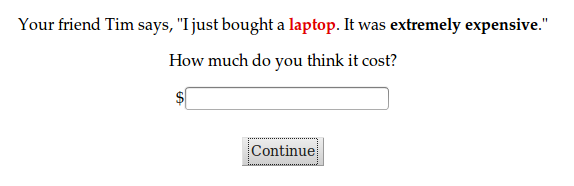
\includegraphics[width=0.6\textwidth]{exp1-q.png}
      \end{center}
      \caption{Screenshot from Experiment 1 target question.} 
      \label{exp1-q}
      \end{figure}

    \subsubsection{Corpus Methods}
      The word frequencies used in our analysis were collected from the Google Web 1T 5-grams database \cite{web1t5gram}\footnote{
      We also ran the same analyses on frequency information collected from the Google Books American Ngrams Corpus \cite{books2011} and found similar results.
      }
      In the analysis below we use word length and word surprisal (negative log-frequency) as proxies for a word's cost, as motivated above.
      The syllable lengths of our intensifiers and the surprisals %\todo[inline]{say what surprisal is and why we care before using it.} 
      were correlated, but not strongly so (r = 0.27).

    \subsubsection{Results}
      If the meaning of an intensifier is stronger for higher cost intensifiers, we would expect to find that as surprisal increases and length in syllables increases, the prices participants give will also increase. We find that this is the case.
      %% what's the alternative hypothesis?

      \begin{figure*}[ht]
      \begin{center}
      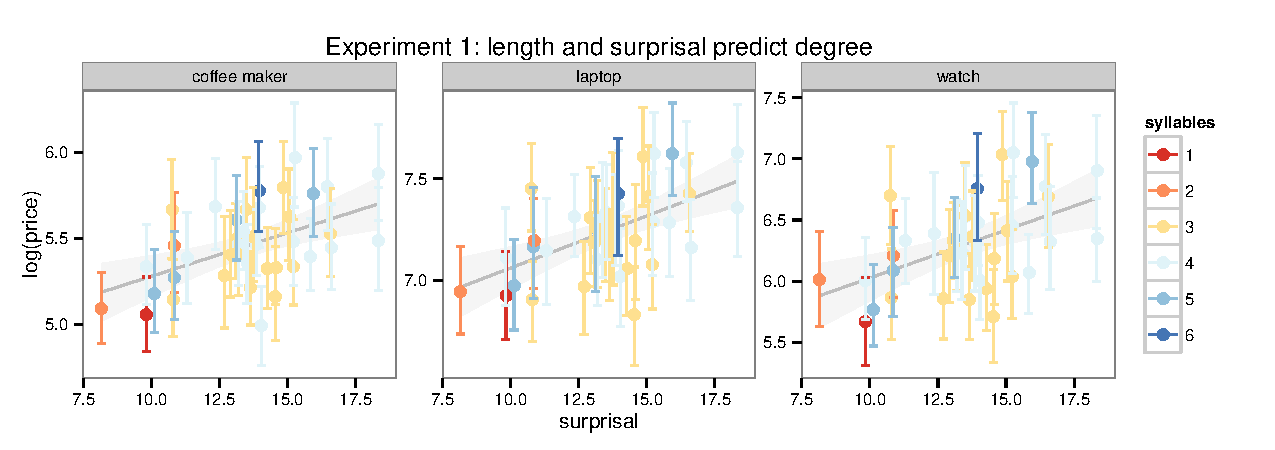
\includegraphics[width=\textwidth]{exp1.pdf}
      \end{center}
      \caption{Results of Experiment 1. As surprisal and length in syllables increase, participants' free response prices increase.} 
      \label{exp1-plot}
      \end{figure*}

      We ran a linear mixed effects regression with centered fixed effects of syllables, surprisal, and their interaction, and random intercepts and slopes for syllables and surprisal for both participant and object.
      We used the logarithm of participants' price estimates as the dependent variable, because of evidence that people's representation of numbers, including prices, is logarithmic \cite[e.g.]{dehaene}\footnote{I.e. the perceptual distance between two prices the same dollar amount apart is more for small numbers (e.g. \$3 and \$6) and less for large numbers (e.g. \$1,543 and \$1,546).}.
      
      Our results are shown in Figure~\ref{exp1-plot}. Both measures of cost play a role in predicting participants' price estimates. We found a significant main effects of surprisal ($\beta=0.0537, SE=0.00935, t(3)=5.74, p<0.05$) such that less frequent words tend to be associated with higher price estimates. We also found a significant main effect of syllable length ($\beta=0.0931, SE=0.0182, t(5)=5.112, p<0.005$), above and beyond surprisal, such that longer words predict stronger meanings. We also found a significant interaction ($\beta=0.0193, SE=0.00515, t(3.5)=3.75, p<0.0005$) between surprisal and syllable length, wich may indicate that the relationship between the two predictors of cost is not simply additive, and that having multiple sources of communicative cost (i.e. length and surprisal) might increase the implicature even more.

      Thus intensifiers that are less frequent and longer (and therefore are more costly to utter) also tend to be interpreted as having stronger meanings, at least when used to modify \emph{expensive}. %Furthermore, the relationship appears to be linear in surprisal and length (though with an interaction), as predicted.
      %This is consistent with the M-implicature model introduced above.
  
  \subsection{Experiment 2}
      The M-implicature account described above implies that there is no semantic interaction between the intensifier and the adjective it is applied to. Instead an intensifier should contribute similar cost, and therefore meaning, to the different adjectival phrases in which it occurs\footnote{If the bigram frequency of the modified adjective (``very expensive'') deviated from that expected based on independent word frequencies our frequency-based cost account would predict an interactive effect on meaning. This would be a relatively small effect, and the relevant bigrams were too sparse in our corpora to pursue.}.
      To explore this issue, we would like to extend our results to additional adjectival scales. However, most scales are not so easily quantifiable as price; we require a different dependent measure in order to probe them.
      For Experiment 2 we used a forced-ranking dependent measure, which allows us to consider additional adjectival scales. This dependent measure has the added benefit of providing a more sensitive measure of the differences in degrees between similar adjectival phrases.

    \subsubsection{Method}
      30 participants with US IP addresses were recruited through Amazon's Mechanical Turk and paid \$0.40 for  participation.

      We asked participants to order (by clicking and dragging) various adjective phrases with the same adjective but different intensifiers according to strength of meaning. Because arranging these phrases required participants to be aware of the full set of adjective phrases and access all of them on the same computer screen (which might vary in size for different participants), not all of our 40 intensifiers could effectively be presented at once. We divided the 40 intensifiers from Experiment 1 into four lists of 10 intensifiers. 
      %(Table~\ref{exp2-intensifiers}).
      Each list was randomly paired with one of four adjectives (\w{old}, \w{expensive}, \w{beautiful}, and \w{tall}).
      For each adjective-list pairing, participants were shown every combination of the 10 intensifiers with one adjective.
      Participants were asked to move the adjective phrases from the left to the right side of the screen, reordering the phrases from the ``lowest'' to the ``highest'' degree (Figure~\ref{exp2-q}).
      Each participant completed four such trials, seeing all four lists and all four adjectives.
      The pairings between list and adjective were randomized between participants.
      The division of the intensifiers into lists of 10 was constant, so that the same 10 intensifiers were always shown together to simplify data analysis.

      \begin{figure}[ht]
      \begin{center}
      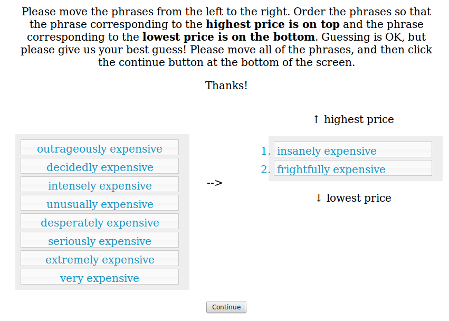
\includegraphics[width=0.4\textwidth]{exp2-q.png}
      \end{center}
      \caption{Screenshot from Experiment 2 target question.} 
      \label{exp2-q}
      \end{figure}
      
    \subsubsection{Results}
      Our results for Experiment 2 are shown in Figure~\ref{exp2-plot}. We ran an ordinal
      regression with centered surprisal and syllable lengths and their interaction as fixed effects.
      As in Experiment 1, we found strong main effects of surprisal ($\beta=0.319, SE=0.0247, t=12.9, p<5e-38$) and syllable length ($\beta=0.437, SE=0.0658, t=6.64, p<5e-11$), with only a trending interaction ($p=0.0825$).
      In other words, we again found that participants assign stronger interpretations to intensifiers with higher surprisals and/or higher syllable lengths, extending now across four different adjectival scales.
      %could say something more about these results? interaction between intensifier and adjective?

      \begin{figure*}[ht]
      \begin{center}
      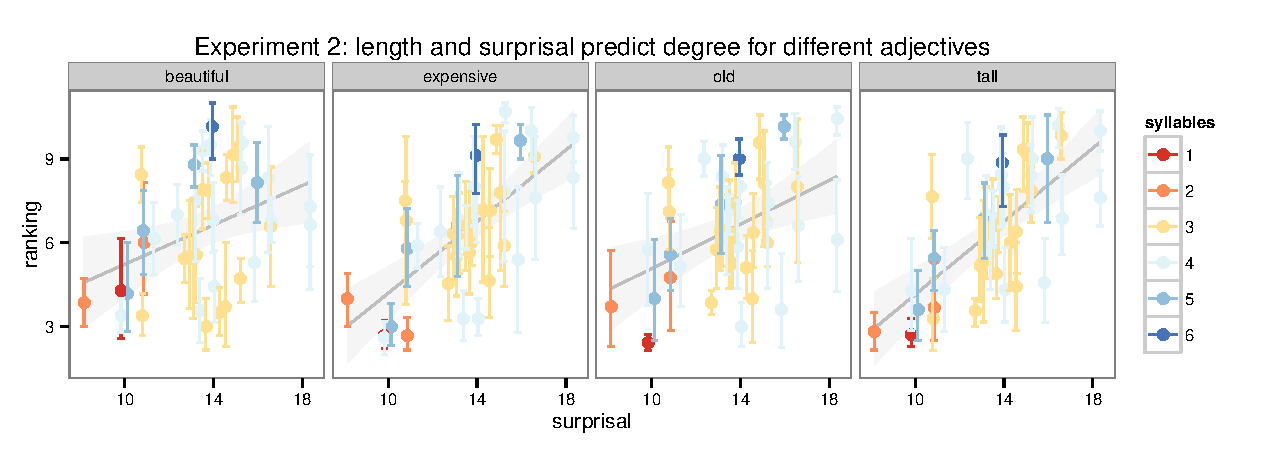
\includegraphics[width=\textwidth]{exp2.pdf}
      \end{center}
      \caption{Results of Experiment 2. As surprisal and length in syllables increase, participants' rankings increased.} 
      \label{exp2-plot}
      \end{figure*}
      
  \subsection{Discussion}    
      In these first two experiments we provided evidence that intensifier meanings depend systematically on the length and frequency of distribution of those word forms.
      While it is unlikely that this accounts for all intensifier meaning, it does suggest that a major portion of meaning comes not from arbitrary, conventional association of signal to sign \cite{saussure}, but from features of the word's form and distribution.

      Since this is a correlational study, such a relationship does not confirm that an intensifier's cost \emph{causes} it to have a given meaning.%This correlation is predicted by the model sketched above, but it might be predicted by other analyses of intensifiers and their meanings.
      Rarity in particular might be correlated with strength of meaning merely because more extreme meanings refer to less probable things in the world, are therefore talked about less, and therefore the words with those meanings will necessarily be rarer.
      %% this next bit is sketch
      Although it seems reasonable to suspect that word frequencies reflect the probabilities of the real-world concepts they describe, it might also be the case that improbable things are more likely to be commented on, and so to a certain extent the frequencies of words that describe rare concepts will be inflated. Syllable length in turn might depend on the frequency or simplicity of a word, either because words that are frequently used gets shortened over time \cite{someone} or because words that refer to simpler or more common concepts enter the lexicon sooner (when more shorter word forms remain unassigned to meanings). It is therefore possible that these measures of cost have no causal influence on the meanings of intensifiers within a particular communicative act.
      
      In order to address the question of whether utterance cost might cause people to interpret an intensifier as stronger, we ran Experiments 3 and 4, where we directly manipulated one of our measures of cost -- length -- in novel intensifiers which have no conventional meaning associated to them.

\section{Manipulation: novel intensifiers of varying lengths}
  \todo{We can directly vary the length of a novel intensifier pretty easily. People will have to guess the meaning, and they might use length as a cue.}

  \subsection{Experiment 3}
    \todo{motivate}

    \subsubsection{Method}
      28 participants with US IP addresses were recruited through Amazon's Mechanical Turk and paid \$0.80 for their participation.

      Experiment 3 was identical to Experiment 1, except that we included only a subset of the intensifiers from Experiment 1\footnote{We chose this subset of 9 intensifiers to get a wide range of surprisals and syllable lengths (\w{colossally}, \w{phenomenally}, \w{mightily}, \w{extraordinarily}, \w{amazingly}, \w{terribly}, \w{notably}, \w{significantly}, \w{quite})} and each participant also saw one novel intensifier, randomly mixed in with the rest.

      We varied the novel intensifier between participants from a set of 6 novel intensifiers, three of which were relatively short (\w{lopusly}, \w{ratumly}, and \w{bugornly}) and three of which shared the same ``root'' but were two CVCV syllables longer (\w{fepolopusly}, \w{gaburatumly}, and \w{tupabugornly}).

      Participants again estimated prices for objects of three different categories paired with all of the intensifiers. The order of the questions was randomized between and within participants.

    \subsubsection{Results}
      In Experiment 3, we included as filler a subset of the intensifiers we tested in Experiment 1, and so we first confirmed our findings from Experiment 1. As in Experiment 1, we ran a linear mixed effects regression with centered fixed effects of syllables, surprisal, and their interaction, and random intercepts and slopes for syllables and surprisal for both participant and object, and we used the logarithm of participants' price estimates as the dependent variable. Replicating our findings from Experiment 1, we found significant main effects of surprisal ($\beta=0.09481$, $SE=0.02503$, $t=3.787$, $p<0.05$) and syllable length ($\beta=0.1622$, $SE=0.02716$, $t=5.972$, $p<0.0005$), and a significant interaction ($\beta=0.03071$, $SE=0.009156$, $t=3.353$, $p<0.005$).

      \begin{figure}[ht]
      \begin{center}
      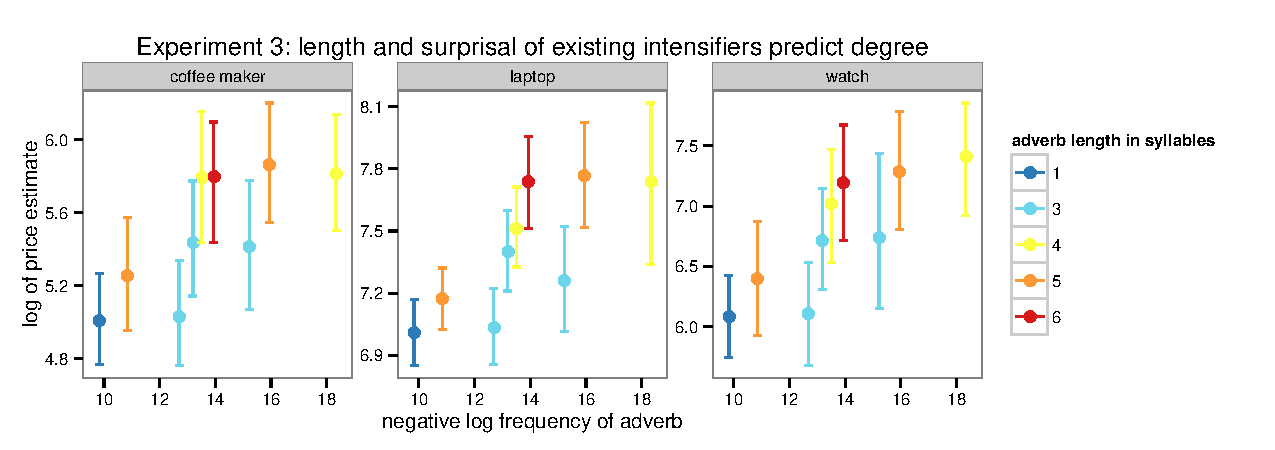
\includegraphics[width=\textwidth]{exp3_replication.pdf}
      \end{center}
      \caption{In Experiment 3, we replicated our findings from Experiment 1.} 
      \label{exp3_replication}
      \end{figure}

      % We have many more data points for existing intensifiers than for novel intensifiers, since we included only one novel adjective for each participant. From these sparse data, it is hard to tell whether interpretations of novel adjectives are as consistent as interpretations of existing ones, though many of the more extreme data points are for novel intensifiers. All responses are shown in figure \ref{exp3_all_responses}.
      % 
      % \begin{figure}[ht]
      % \begin{center}
      % 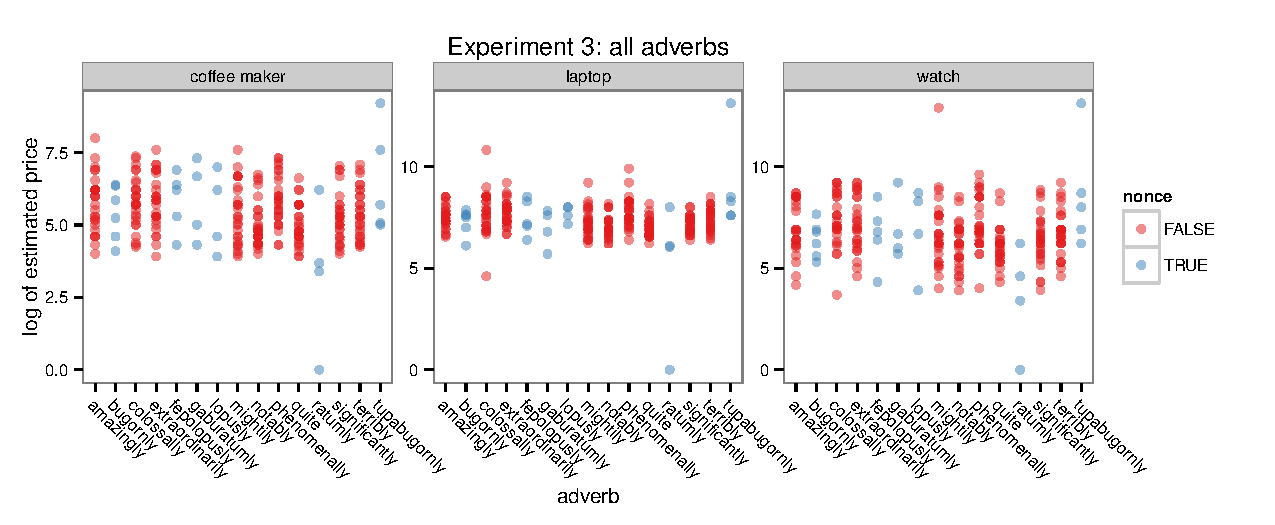
\includegraphics[width=\textwidth]{free_response_all_intensifiers.pdf}
      % \end{center}
      % \caption{Novel intensifiers are in blue and existing intensifiers are in red.} 
      % \label{exp3_all_responses}
      % \end{figure}

      We then ran a linear mixed effects model on only the novel intensifiers, with length (``long'' or ``short'') as a fixed effect, random intercepts and slopes for objects, and random intercepts for the three different ``roots''. We found a significant effect of length condition ($\beta(\mbox{``short''})=-1.3955$, $SE=0.3794$, $t=-3.678$, $p<0.0005$), indicating that people use the length of an intensifier in the moment in order to interpret its meaning, even for novel intensifiers with no conventional meaning.

      \begin{figure}[ht]
      \begin{center}
      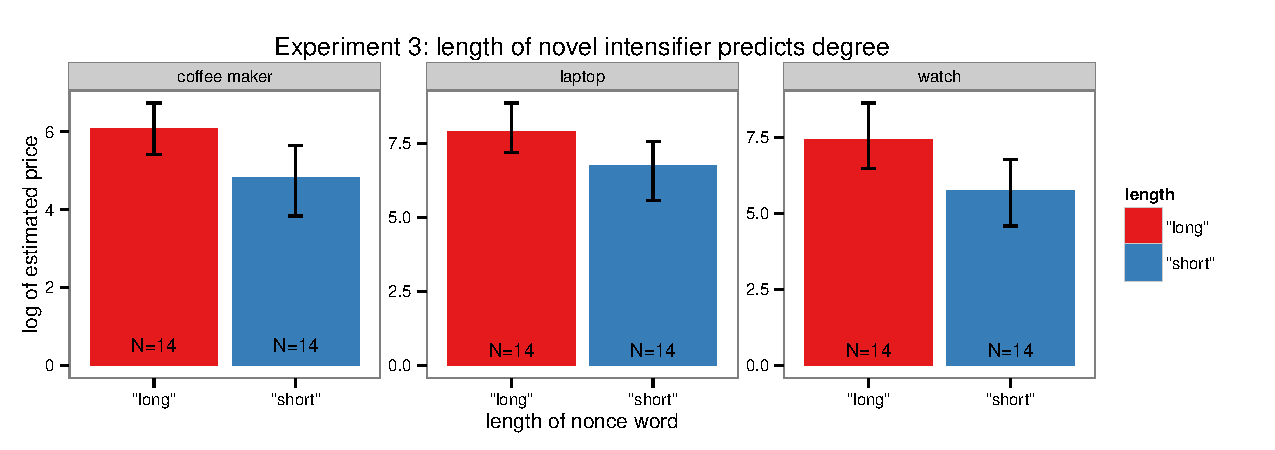
\includegraphics[width=\textwidth]{free_response_nonce_intensifiers_length.pdf}
      \end{center}
      \caption{In Experiment 3, we found a significant effect of length for all novel intensifiers.} 
      \label{exp3_novel}
      \end{figure}

  \subsection{Experiment 4}
    \todo{motivate}

    \subsubsection{Method}
      X participants with US IP addresses were recruited through Amazon's Mechanical Turk and paid \$0.X0 for their participation.
      
      Experiment 3 was identical to Experiment 2, except that we included only two of the four adjectives (\w{expensive} and \w{tall}) -- which we varied \emph{between} participants -- and the intensifiers from Experiment 3. Each participant saw exactly one novel intensifier, and we varied the novel intensifier between participants.
      
      As in Experiment 2, participants were asked to drag and drop adjective phrases into order from highest to lowest on the adjectival scale. However, in Experiment 4, each participant saw exactly one of two adjectives (\w{expensive} or \w{tall}, varied between participants) and only the set of intensifiers from Experiment 3. This set included one novel intensifier, which we varied between participants. As in Experiment 2, adjective phrases for each intensifier-adjective pairing were initialized in random order.

    \subsubsection{Results}
      With our filler intensifiers for Experiment 4, we replicating our findings from Experiment 2 of significant effects of both surprisal ($\beta=0.781$, $SE=0.0499$, $t=15.7$, $p<5e-16$)
      and syllable length ($\beta=1.111$, $SE=0.0974$, $t=11.4$, $p<5e-16$) on the order in the list that participants chose for the intensifiers.
      In this replication, we also found a significant
      interaction ($\beta=0.189$, $SE=0.0351$, $t=5.39$, $p<5e-7$). This is consistent with the findings from all of our previous experiments.
      
      For the novel intensifiers, we ran an ordinal regression on the rankings (relative to the filler intensifiers) and found a significant effect of length condition ($\beta(\mbox{``short''})=-1.17$, $SE=0.525$, $t=-2.24$, $p<0.05$).

    \subsection{Discussion}
      Overall, in Experiments 3 and 4 we found that length is a significant predictor of interpretation strength for novel intensifiers. These novel intensifiers have no established meaning, so the relationship between their length and strength cannot simply be a function of \todo{what's a succinct way of saying the alternative?}. At least some inference must happen online as people see these words that influences their interpreations.
      
      \todo{It's unclear whether this inference is pragmatic meta-linguistic, but either way, it's an online inference.}
  
\section{General discussion}
  \todo{Longer, rarer (more costly to utter) intensifiers tend to have stronger meanings, and people can use utterance cost information, like length, to interpret intensifiers. This might be a large source of intensifiers' meanings.}

\bibliographystyle{plain}

\bibliography{intensifiers}

\end{document}
